\documentclass[tikz,border=6pt]{standalone}
\usepackage{amsmath,amssymb}
\definecolor{inD}{RGB}{31,94,165}\definecolor{inC}{RGB}{214,96,33}
\tikzset{
  m/.style={circle,inner sep=0pt,minimum size=9pt,ball color=inD!85,draw=inD!60!black,line width=0.3pt},
  c/.style={circle,inner sep=0pt,minimum size=9pt,ball color=inC!90,draw=inC!60!black,line width=0.3pt},
  lab/.style={font=\small,fill=white,fill opacity=0.85,text opacity=1,inner sep=1.2pt,rounded corners=1pt},
  e/.style={line width=0.75pt,black!55},
  ec/.style={line width=1.4pt,inC!80!black},
  ex/.style={line width=0.6pt,black!35,densely dashed}}
\begin{document}

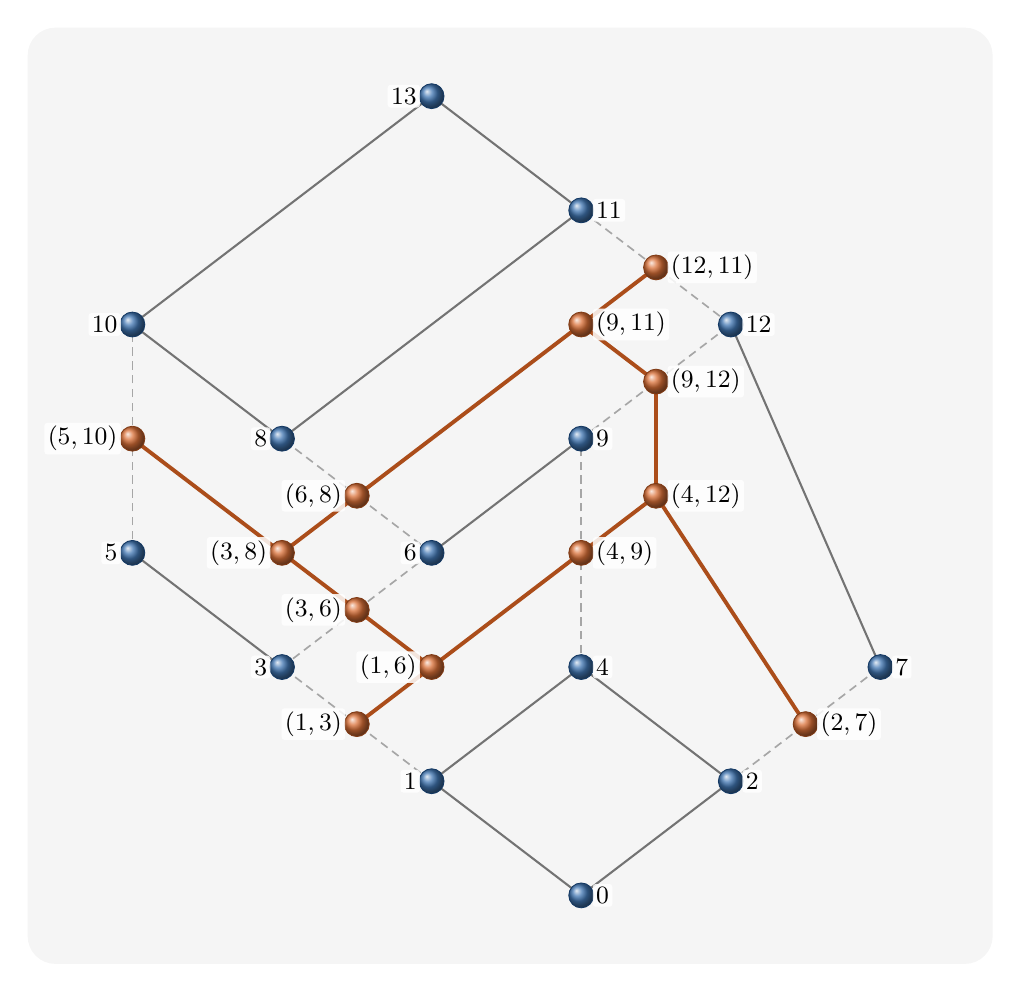
\begin{tikzpicture}[x=1.9cm,y=1.45cm]
\fill[black!4,rounded corners=10pt] (-3.7,-0.6) rectangle (2.75,7.6);
\coordinate (d0) at (0.000,0.000);
\coordinate (d1) at (-1.000,1.000);
\coordinate (d2) at (1.000,1.000);
\coordinate (p1x3) at (-1.500,1.500);
\coordinate (p2x7) at (1.500,1.500);
\coordinate (p1x6) at (-1.000,2.000);
\coordinate (d3) at (-2.000,2.000);
\coordinate (d4) at (0.000,2.000);
\coordinate (d7) at (2.000,2.000);
\coordinate (d5) at (-3.000,3.000);
\coordinate (p3x6) at (-1.500,2.500);
\coordinate (p3x8) at (-2.000,3.000);
\coordinate (p4x9) at (0.000,3.000);
\coordinate (d6) at (-1.000,3.000);
\coordinate (p4x12) at (0.500,3.500);
\coordinate (p5x10) at (-3.000,4.000);
\coordinate (p6x8) at (-1.500,3.500);
\coordinate (d8) at (-2.000,4.000);
\coordinate (d9) at (0.000,4.000);
\coordinate (d10) at (-3.000,5.000);
\coordinate (p9x12) at (0.500,4.500);
\coordinate (d12) at (1.000,5.000);
\coordinate (p9x11) at (0.000,5.000);
\coordinate (p12x11) at (0.500,5.500);
\coordinate (d11) at (0.000,6.000);
\coordinate (d13) at (-1.000,7.000);
\draw[ec] (p1x3) -- (p1x6);
\draw[ec] (p2x7) -- (p4x12);
\draw[ec] (p1x6) -- (p3x6);
\draw[ec] (p1x6) -- (p4x9);
\draw[ec] (p3x6) -- (p3x8);
\draw[ec] (p3x8) -- (p5x10);
\draw[ec] (p3x8) -- (p6x8);
\draw[ec] (p4x9) -- (p4x12);
\draw[ec] (p4x12) -- (p9x12);
\draw[ec] (p6x8) -- (p9x11);
\draw[ec] (p9x12) -- (p9x11);
\draw[ec] (p9x11) -- (p12x11);
\draw[ex] (d1) -- (p1x3);
\draw[ex] (d2) -- (p2x7);
\draw[ex] (p1x3) -- (d3);
\draw[ex] (p2x7) -- (d7);
\draw[ex] (d3) -- (p3x6);
\draw[ex] (d4) -- (p4x9);
\draw[ex] (d5) -- (p5x10);
\draw[ex] (p3x6) -- (d6);
\draw[ex] (p4x9) -- (d9);
\draw[ex] (d6) -- (p6x8);
\draw[ex] (p5x10) -- (d10);
\draw[ex] (p6x8) -- (d8);
\draw[ex] (d9) -- (p9x12);
\draw[ex] (p9x12) -- (d12);
\draw[ex] (d12) -- (p12x11);
\draw[ex] (p12x11) -- (d11);
\draw[e] (d0) -- (d1);
\draw[e] (d0) -- (d2);
\draw[e] (d1) -- (d4);
\draw[e] (d2) -- (d4);
\draw[e] (d3) -- (d5);
\draw[e] (d7) -- (d12);
\draw[e] (d6) -- (d9);
\draw[e] (d8) -- (d10);
\draw[e] (d8) -- (d11);
\draw[e] (d10) -- (d13);
\draw[e] (d11) -- (d13);
\node[m] at (d0) {}; \node[lab,right=4pt] at (d0) {$0$};
\node[m] at (d1) {}; \node[lab,left=4pt] at (d1) {$1$};
\node[m] at (d2) {}; \node[lab,right=4pt] at (d2) {$2$};
\node[c] at (p1x3) {}; \node[lab,left=4pt] at (p1x3) {$(1,3)$};
\node[c] at (p2x7) {}; \node[lab,right=4pt] at (p2x7) {$(2,7)$};
\node[c] at (p1x6) {}; \node[lab,left=4pt] at (p1x6) {$(1,6)$};
\node[m] at (d3) {}; \node[lab,left=4pt] at (d3) {$3$};
\node[m] at (d4) {}; \node[lab,right=4pt] at (d4) {$4$};
\node[m] at (d7) {}; \node[lab,right=4pt] at (d7) {$7$};
\node[m] at (d5) {}; \node[lab,left=4pt] at (d5) {$5$};
\node[c] at (p3x6) {}; \node[lab,left=4pt] at (p3x6) {$(3,6)$};
\node[c] at (p3x8) {}; \node[lab,left=4pt] at (p3x8) {$(3,8)$};
\node[c] at (p4x9) {}; \node[lab,right=4pt] at (p4x9) {$(4,9)$};
\node[m] at (d6) {}; \node[lab,left=4pt] at (d6) {$6$};
\node[c] at (p4x12) {}; \node[lab,right=4pt] at (p4x12) {$(4,12)$};
\node[c] at (p5x10) {}; \node[lab,left=4pt] at (p5x10) {$(5,10)$};
\node[c] at (p6x8) {}; \node[lab,left=4pt] at (p6x8) {$(6,8)$};
\node[m] at (d8) {}; \node[lab,left=4pt] at (d8) {$8$};
\node[m] at (d9) {}; \node[lab,right=4pt] at (d9) {$9$};
\node[m] at (d10) {}; \node[lab,left=4pt] at (d10) {$10$};
\node[c] at (p9x12) {}; \node[lab,right=4pt] at (p9x12) {$(9,12)$};
\node[m] at (d12) {}; \node[lab,right=4pt] at (d12) {$12$};
\node[c] at (p9x11) {}; \node[lab,right=4pt] at (p9x11) {$(9,11)$};
\node[c] at (p12x11) {}; \node[lab,right=4pt] at (p12x11) {$(12,11)$};
\node[m] at (d11) {}; \node[lab,right=4pt] at (d11) {$11$};
\node[m] at (d13) {}; \node[lab,left=4pt] at (d13) {$13$};
\end{tikzpicture}
\end{document}
